\documentclass[xcolor=pdftex,dvipsnames,table,mathserif]{beamer}
\usetheme{default}
%\usetheme{Darmstadt}
%\usepackage{times}
%\usefonttheme{structurebold}

\usepackage[english]{babel}
%\usepackage[table]{xcolor}
\usepackage{pgf,pgfarrows,pgfnodes,pgfautomata,pgfheaps}
\usepackage{amsmath,amssymb,setspace}
\usepackage[latin1]{inputenc}
\usepackage[T1]{fontenc}
\usepackage{relsize}
\usepackage[absolute,overlay]{textpos} 
\newenvironment{reference}[2]{% 
  \begin{textblock*}{\textwidth}(#1,#2) 
      \footnotesize\it\bgroup\color{red!50!black}}{\egroup\end{textblock*}} 

\DeclareMathSizes{10}{10}{6}{6} 


\title [Homogenous Products]{Homogenous Products}
\author{C.Conlon}
\institute{Grad IO }
\date{Fall 2016}
\setbeamerfont{equation}{size=\tiny}
\begin{document}

\begin{frame}
\titlepage
\end{frame}

\begin{frame}{Introduction}
One of the earliest exercises in econometrics is the estimation of supply and demand for a homogenous product
\begin{itemize}
\item According to Stock and Trebbi (2003) IV regression first appeared in a book by Phillip G. Wright in 1928 entitled \textit{The Tariff on Animal and Vegetable Oils} [neatly tucked away in Appendix B:  Supply and Demand for Butter and Flaxseed.]
\item Lots of similar studies of simultaneity of supply + demand for similar agricultural products or commodities.
\end{itemize}
\end{frame}

\begin{frame}{Working (1927)}
Supply and Demand For Coffee, everything is linear
\begin{eqnarray*}
Q_t^d &=& \alpha_0 + \alpha_1 P_t + U_t\\
Q_t^d &=& \beta_0 + \beta_1 P_t + V_t\\
Q_t^d &=& Q_t^s
\end{eqnarray*}
Solving for $P_t,Q_t$:
\begin{eqnarray*}
P_t &=& \frac{\beta_0 - \alpha_0}{\alpha_1 - \beta_1} + \frac{V_t - U_t}{\alpha_1 - \beta_1}\\
Q_t &=& \frac{\alpha_1 \beta_0 - \alpha_0 \beta_1}{\alpha_1 - \beta_1} + \frac{\alpha_1 V_t - \beta_1 U_t}{\alpha_1 - \beta_1}
\end{eqnarray*}
Price is a function of both error terms, and we can't use a clever substitution to cancel things out.
\end{frame}

\begin{frame}{Working (1927)}
To make things really obvious:
\begin{eqnarray*}
Cov(P_t,U_t) = - \frac{Var(U_t)}{\alpha_1 -\beta_1} \\
Cov(P_t,V_t) =  \frac{Var(V_t)}{\alpha_1 -\beta_1} 
\end{eqnarray*}
\begin{itemize}
\item When demand slopes down ($\alpha_1 < 0)$ and supply slopes up $(\beta_1 > 0)$ then price is positively correlated with demand shifter $U_t$ and negatively correlated with supply shifter $V_t$.
\end{itemize}
\end{frame}

\begin{frame}{Working (1927)}
\begin{eqnarray*}
Cov(P_t, Q_t) &=& \alpha_1 Var P_t + Cov (P_t,U_t)\\
Cov(P_t, Q_t) &=& \beta_1 Var P_t + Cov (P_t,V_t)
\end{eqnarray*}
\begin{itemize}
\item Bias in OLS estimate (Demand) $Bias(\alpha_1) = \frac{Cov(P_t,U_t)}{Var P_t}$.
\item Bias in OLS estimate (Supply) $Bias(\beta_1) = \frac{Cov(P_t,V_t)}{Var P_t}$.
\item We can actually write both this way when $Cov(U_t,V_t) = 0$:
\begin{eqnarray*}
\text{OLS Estimate }= \frac{\alpha_1 Var(V_t) + \beta_1 Var (U_t)}{Var (V_t) + Var (U_t)}
\end{eqnarray*}
\item More variation in supply $V_t \rightarrow$ better estimate of demand.
\item More variation in demand $U_t \rightarrow$ better estimate of supply.
\item Led Working to say the \alert{statistical demand function} (OLS) is not informative about the economic demand function (or supply function).
\end{itemize}
\end{frame}

\begin{frame}{Simultaneity}
\begin{itemize}
\item For most of you, this was probably a review.
\item We know what the solution is going to be to the simultaneity problem.
\item We need an \alert{excluded instrument} that shifts one curve without affecting the other.
\item We can use this to form a 2SLS estimate.
\item Instead let's look at something a little different...
\end{itemize}
\end{frame}


\begin{frame}{Simultaneity and Identification}
Angrist, Imbens, and Graddy (ReStud 2000).
\begin{itemize}
\item Demand for Whiting (fish) at Fulton Fish Market
\item Do not place functional form restrictions on demand (log-log, log-linear, linear, etc.).
\item ``What does linear IV regression of $Q$ on $P$ identify, even if the true (but unknown) demand function is nonlinear''
\item Takes a program evaluation/treatment effects approach to understanding the ``causal effect'' of price on quantity demanded.
\item Aside: Is there even such a thing as the causal effect of price on quantity demanded?
\end{itemize}
\end{frame}

\begin{frame}{Four Cases}
Ranked in increasing complexity
\small
\begin{enumerate}
\item Linear system with constant coefficients
\begin{eqnarray*}
q_t^d(p,z,x) &=& \alpha_0 + \alpha_1 p + \alpha_2 z + \alpha_3 x + \epsilon_t \\
q_t^s(p,z,x) &=& \beta_0 + \beta_1 p + \beta_2 x + \beta_3 x + \eta_t
\end{eqnarray*}
\item Linear system with non-constant coefficients
\begin{eqnarray*}
q_t^d(p,z,x) &=& \alpha_{0t} + \alpha_{1t} p + \alpha_{2t} z + \alpha_{3t} x + \epsilon_t \\
q_t^s(p,z,x) &=& \beta_{0t} + \beta_{1t} p + \beta_{2t} x + \beta_{3} x + \eta_t
\end{eqnarray*}
\item Nonlinear system with constant shape (separable)
\begin{eqnarray*}
q_t^d(p,z,x) &=& q^d(p,z,x)+ \epsilon_t \\
q_t^s(p,z,x) &=& q^s(p,z,x)+ \eta_t
\end{eqnarray*}
\item Nonlinear system with time-varying shape (non-separable)
\begin{eqnarray*}
q_t^d(p,z,x) &=& q^d(p,z,x,\epsilon_t) \\
q_t^s(p,z,x) &=& q^s(p,z,x,\eta_t)
\end{eqnarray*}
\end{enumerate}
\end{frame}

\begin{frame}{AIG: Heterogeneity}
Two kinds:
\begin{enumerate}
\item Heterogeneity depending on value of $p$ fixing $t$ (only relevant in nonlinear models)
\item Heterogeneity across $t$, fixing $p$ (cases 2 and 4).
\end{enumerate}
\begin{itemize}
\item The problem is that we don't generality know which kind of heterogeneity we face.
\item Is case (4) hopeless? Or what can we expect to learn?
\item Even econometricians struggle with non-linear non-separable models (!)
\end{itemize}
\end{frame}

\begin{frame}{AIG: Assumptions}
Assume binary instrument $z_{t} \in \{0,1\}$ to make things easier.

\begin{enumerate}
\item Regularity conditions on $q_t^d, q_t^s,p_t,z_t,w_t$ first and second moment and is stationary, etc.
\begin{itemize}
\item  $q_t^d(p,z,x)$ ,  $q_t^s(p,z,x)$ are continuously differentiable in $p$.
\end{itemize}
\item $z_t$ is a valid instrument in $q_t^d$
\begin{itemize}
\item Exclusion: for all $p,t$ 
\begin{eqnarray*}
q_t^d(p,z=1,x_t) = q_t^d(p,z=0,x_t) \equiv q_t^d(p,x_t)
\end{eqnarray*}
ie: conditioning on $p_t$ means no dependence on $z_t$
\item Relevance: for some period $t$: $q_t^s(p_t,1,x_t) \neq q_t^s(p_t,0,x_t)$.\\
ie: $z_t$ actually shifts supply somewhere!
\item Independence: $\epsilon_t, \eta_t, z_t$ are mutually independent conditional on $x_t$.
\end{itemize}
\end{enumerate}
\end{frame}

\begin{frame}{Wald Estimator}
Focus on the simple case:
\begin{itemize}
\item $z \in \{0,1\}$ where $1$ denotes ``stormy at sea'' and 0 denotes ``calm at sea''
\item Idea is that offshore weather makes fishing more difficult but doesn't change onshore demand.
\item Ignore $x$ (for now at least) or assume we condition on each value of $x$.
\end{itemize}
\begin{eqnarray*}
\hat{\alpha}_{1,0}  \rightarrow^p \frac{E[q_t | z_t] - E[q_t | z_t=0]}{E[p_t | z_t=1] - E[p_t | z_t =0]} \equiv \alpha_{1,0}
\end{eqnarray*}
\begin{itemize}
\item If we are in case (1) then we are good. In fact, any IV gives us a consistent estimate of $\alpha_1$
\item If we are in case (4) then $\alpha_{1,0}$ the object we recover, is not an estimator of a structural parameter.
\item Moreover, this is at best a LATE, and thus it differs depending on which instrument we use!
\end{itemize}
\end{frame}


\begin{frame}{AGI: Negative Results}
\begin{itemize}
\item Should we divorce structural estimation from estimating ``deep'' population parameters (as suggested by Lucas critique)?
\item Authors make the point that IV estimator identifies something about relationship between $p$ and $q$, without identifying deep structural parameters?
\item In IO this is a somewhat heretical idea (especially to start the course with).
\end{itemize}
\end{frame}

\begin{frame}{AGI: Structural Interpretation}
In order to interpret the Wald estimator $\alpha_{1,0}$ we make some additional \alert{economic} assumptions on the structure of the problem:
\begin{enumerate}
\item Observed price is market clearing price $q_t^d(p_t) = q_t^s(p_t,z_t)$ for all $t$. (This means no frictions!).
\item ``Potential prices'': for each value of $z$ there is a unique market clearing price
\begin{eqnarray*}
\forall z,t : \tilde{p}(z,t) \mbox{ s.t. } q_t^d(\tilde{p}(z,t)) = q_t^s(\tilde{p}(z,t),z).
\end{eqnarray*}
\end{enumerate}
$\tilde{p}(z,t)$ is the potential price under any counterfactual $(z,t)$
\end{frame}


\begin{frame}{AGI: Structural Interpretation}
\begin{itemize}
\item Just like in IV we need denominator to be nonzero so that
$E[p_t | z_t=1] \neq E[p_t | z_t = 0]$.
\item Other key assumption is the familiar \alert{monotonicity} assumption
\begin{itemize}
\item $\tilde{p}(z,t)$ is weakly increasing in $z$.
\item Just like in program evaluation this is the key assumption. There it rules out ``defiers'' here it allows us to interpret the \alert{average slope} as $\alpha_{1,0}$.
\item Assumption is untestable because you do not observe both potential outcomes $\tilde{p}(0,t)$ and $\tilde{p}(1,t)$ (same as in program evaluation).
\item Any story about IV is just a story! (Always the case!) unless we have repeated observations on the same individual.
\end{itemize}
\end{itemize}
\end{frame}


\begin{frame}{AGI: Lemma 1}
The key result establishes that the numerator of $\alpha_{1,0}$:
\begin{eqnarray*}
E[q_t | z_t =1] - E[q_t | z_t = 0] = E_t \left[\int_{\tilde{p}(0,t)}^{\tilde{p}(1,t)} \frac{\partial q_t^d(s)}{\partial s}{d\, s} \right]
\end{eqnarray*}
\begin{itemize}
\item For each $t$ we average over the slope of demand curve among the two potential prices: $\int_{\tilde{p}(0,t)}^{\tilde{p}(1,t)} \frac{\partial q_t^d(s)}{\partial s}{d\, s}$ 
\item This range could differ for each $t$.
\item Then we average this average over all $t$.
\end{itemize}
\end{frame}

\begin{frame}{AGI: Figure}
\begin{figure}
\begin{center}
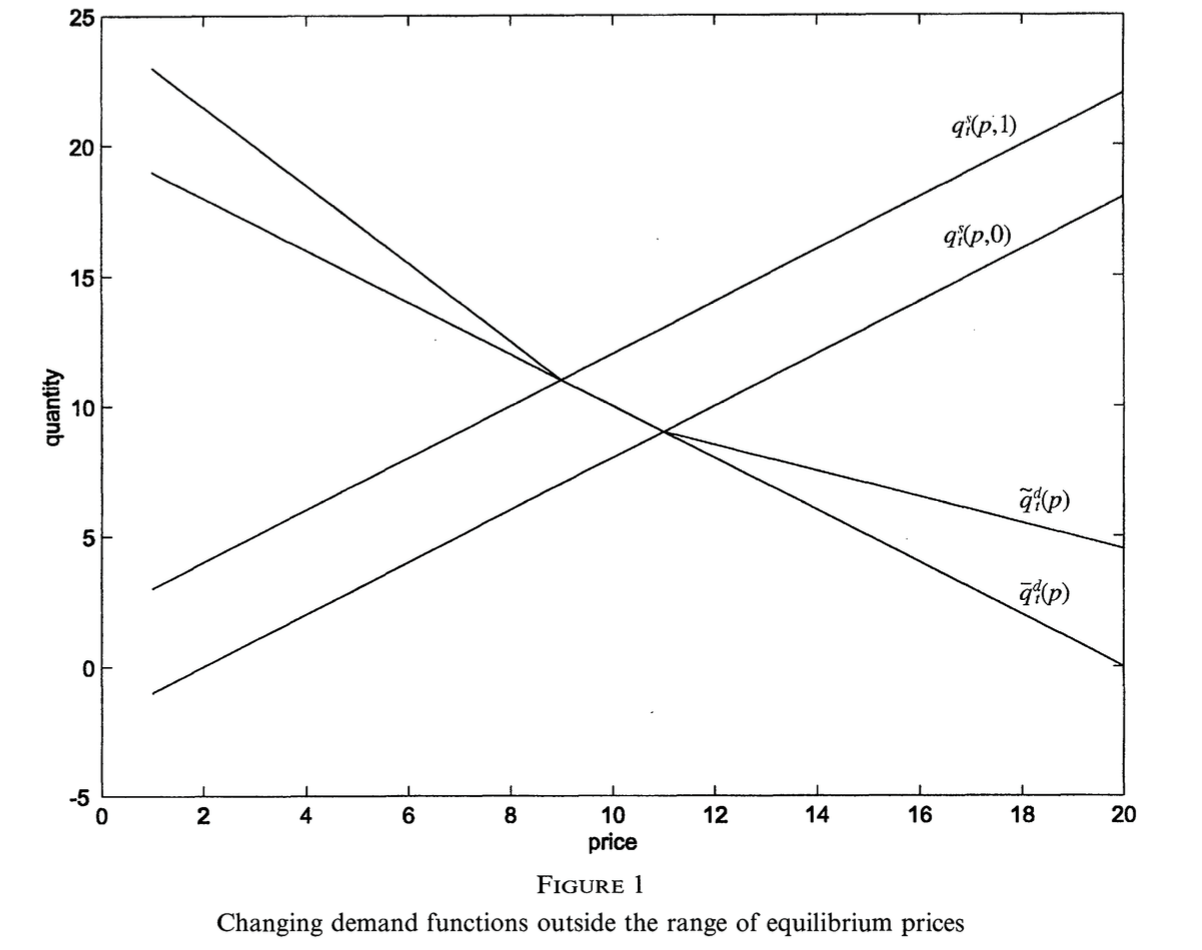
\includegraphics[width=4in]{resources/fishfigure.png}
\end{center}
\end{figure}
\end{frame}

\begin{frame}{AGI: Takeaways}
What did we learn?
\begin{itemize}
\item $\alpha_{1,0}$ only provides information about demand curve in range of potential price variation induced by the instrument.
\item Don't know anything about demand curve outside this range!
\item For different instruments $z$, $\alpha_{1,0}$ has a different interpretation like the LATE does. (Different from the linear model where anything works!).
\item This is a bit weird: different cost shocks could trace out different paths along the demand curve-- why do we care if price change came from a tax change or an input price change? Are they tracing out different subpopulations?
\item We need monotonicity so that we know the range of integration $\tilde{p}(0,t) \rightarrow \tilde{p}(1,t)$ instead of $\tilde{p}(1,t) \rightarrow \tilde{p}(0,t)$
\item Observations where $\tilde{p}(0,t) = \tilde{p}(1,t)$ don't factor into the average but we don't know what these observations are because potential prices are unobserved! What is the relevant sub-sample?
\end{itemize}
\end{frame}




\begin{frame}{AGI: Nonlinear IV}
\begin{eqnarray*}
\alpha_{1,0} &=& \frac{E [ \int_{\tilde{p}(0,t)}^{\tilde{p}(1,t)} \frac{\partial q_t^d(s)}{\partial s} d\, s]}{E \tilde{p}(1,t)- E\tilde{p}(0,t)}\\
 &\rightarrow& \int_0^{\infty} E\left[ \frac{\partial q_t^d(s)}{\partial s} | s \in [\tilde{p}(0,t),\tilde{p}(1,t)]\right ] \omega(s) d  s
\end{eqnarray*}

\begin{itemize}
\item given $t$ average the slope of $q_t^d$ from $\tilde{p}(0,t)$ to $\tilde{p}(1,t)$
\item given price $s \in [\tilde{p}(0,t) ,\tilde{p}(1,t)]$ average $q_t^d(s)$ across $t$. (randomness is due to $\epsilon_t$).
\item Weight $\omega(s)$ is not a function of $t$ but it is largest for prices most likely to fall between $\tilde{p}(0,t)$ and $\tilde{p}(1,t)$.
\item Case (2): $q_t^d(p) = \alpha_{0t} + \alpha_{1t} p + \epsilon_t$.
\begin{eqnarray*}
\alpha_{1,0} = \frac{E[\alpha_{1t} (\tilde{p}(1,t) - \tilde{p}(0,t))]}{E \tilde{p}(1,t) - E \tilde{p}(0,t)} \neq E \alpha_{1,t}
\end{eqnarray*}
We need mean independence
\end{itemize}
\end{frame}


\begin{frame}{AGI: Nonlinear IV}
\begin{itemize}
\item Suppose we had a continuous $z$ instead, now we can do a full nonparametric IV estimator.
\begin{eqnarray*}
a(z) = \lim_{\nu \rightarrow 0} \frac{E(q_t | z) - E(q_t | z-\nu)}{E(p_t | z) - E(p_t | z- \nu)}
\end{eqnarray*}
\item Use a kernel to estimate $\hat{q}|z$ and $\hat{p}|z$
\begin{eqnarray*}
\alpha'(z) =\frac{\hat{q}'(z)}{\hat{p}'(z)} \approx \frac{\hat{q}'(z+h) - \hat{q}(z)}{\hat{p}'(z+h) - \hat{p}(z)}
\end{eqnarray*}
\end{itemize}
\end{frame}



\begin{frame}{AGI: Takeaways}
\begin{itemize}
\item When you have a parametric model, you don't need these results because we can define whatever (nonlinear) parametric functional form we want.
\item There we will focus on parsimonious and realistic parametric functional forms. (this is the rest of the course)
\item If we don't have a parametric model, then these show us that linear IV estimators give us some average (a particular one!) of slopes.
\item Caveat: this only works for a single product. In the multi-product case things are a lot more complicated
\begin{itemize}
\item For multiproduct oligopoly it is much harder to satisfy the \alert{monotonicity} condition.  Why?
\end{itemize}
\end{itemize}
\end{frame}


\end{document}













































